\chapter{Ergebnisse}

Die Klassifizierung des Zustandes der menschlichen Retina anhand von OCT
Aufnahmen in 4 Klassen (gesund + 3 Erkrankungen) lässt sich mit Hilfe des
maschinellen Lernens mit einer Genauigkeit von bis zu $\SI{90}{\percent}$
durchführen. Eine Lösung dieser Aufgabe, wie sie in dieser Arbeit beschrieben
ist, erfordert allerdings eine sehr hohe Rechenkapazität. Der verwendete
Datensatz liefert mit etwa $90\,000$ Bildern in sehr guter Auflösung eine
ausreichende Statistik, um gute Ergebnisse zu erzielen.
Die Hauptarchitektur eines CNN zeigt hierbei mit Abstand die beste
\textit{performance}. Nach etwa 40 Epochen lässt sich mit diesem Netz ein
Modell generieren, welches 4 Klassen mit einer Genauigkeit von
$\SI{90}{\percent}$ unterscheiden kann. Durch die Architektur können so Bilder
verschiedener Größen und Datensätze unterschiedlicher Verteilungen zur
Vorhersage verwendet werden. Durch ausreichende Regularisierung treten keine
Effekte von \textit{overtraining} auf, wie in Abbildung~\ref{fig:hist} zu sehen
ist.
%
\begin{figure}[h!]
  \subcaptionbox{Genauigkeit\label{fig:gen}}{\centering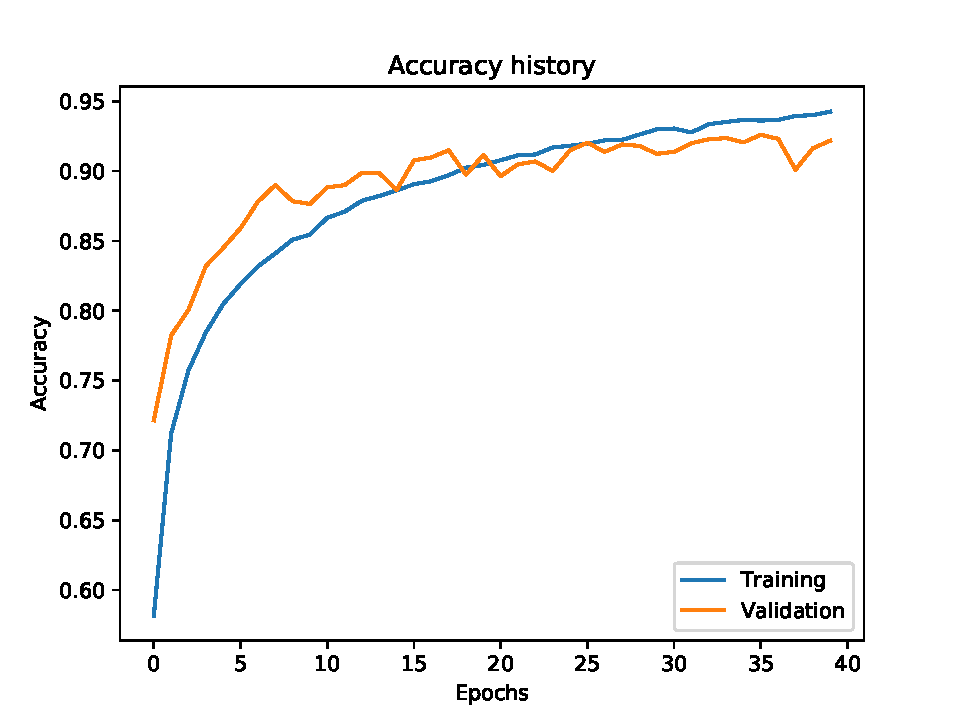
\includegraphics[width=0.5\linewidth]{Plots/accuracy_history_smaller.pdf}}
  \subcaptionbox{Verlustfunktion\label{fig:lo}}{\centering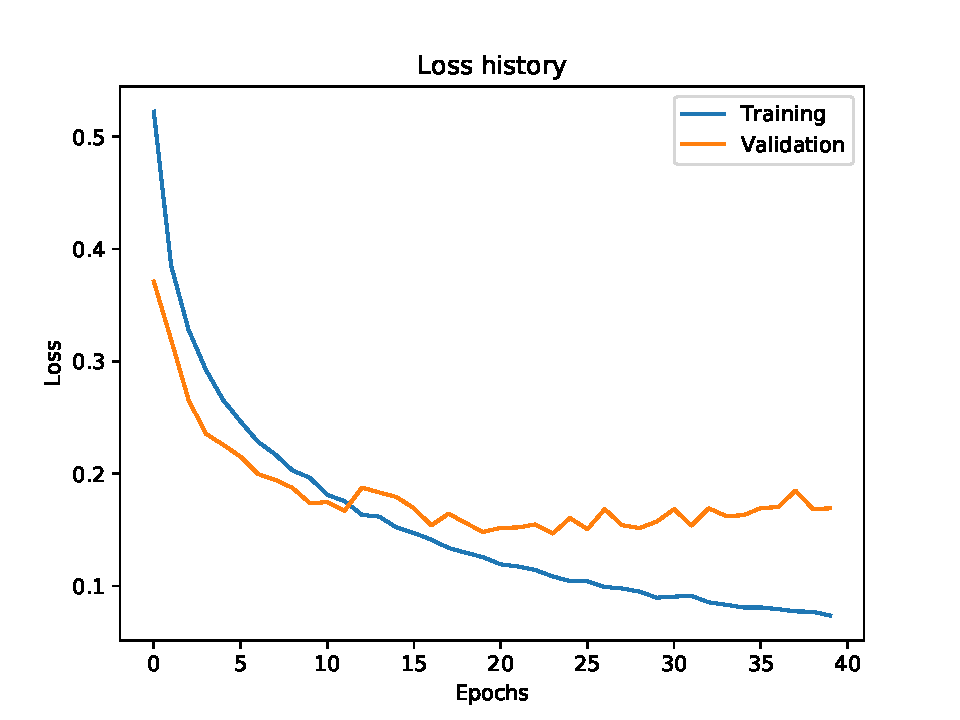
\includegraphics[width=0.5\linewidth]{Plots/loss_history_smaller.pdf}}
  \caption{Die Genauigkeit \protect\subref{fig:gen}, sowie die Verlustfunktion \protect\subref{fig:lo} der Hauptarchitektur des CNN. Es zeigen sich hier nach 40 Epochen keine Anzeichen für ein \textit{overtraining}.}
  \label{fig:hist}
\end{figure}
%
Betrachtet man Beispiele für die Klassen CNV, DRUSEN und NORMAL, deren
Trennung für das Netz am schwierigsten ist, so fällt auf, dass es sich hierbei
um Bilder handelt, die auch für Menschen schwierig zu trennen sind. Das Netz
erreicht allerdings mit der oben beschriebenen Genauigkeit eine Präzesion, die
weit über der eines ungelernten Auges reicht. Ärzte hingegen erreichen
Genauigkeiten, die noch über dem hier erreichten Wert liegen.\\
Eine Genauigkeit von $\SI{90}{\percent}$ durch Bilderkennung auf 4 Klassen zu
erreichen, stellt allerdings eine sehr optimistisch stimmende Leistung dar.
Besonders in der Medizin können solche Anwendungen auch eine äußerst praktische
Anwendung finden.
\newpage
%
\begin{figure}[h!]
  \subcaptionbox{Verwirrungsmatrix\label{fig:conf}}{\centering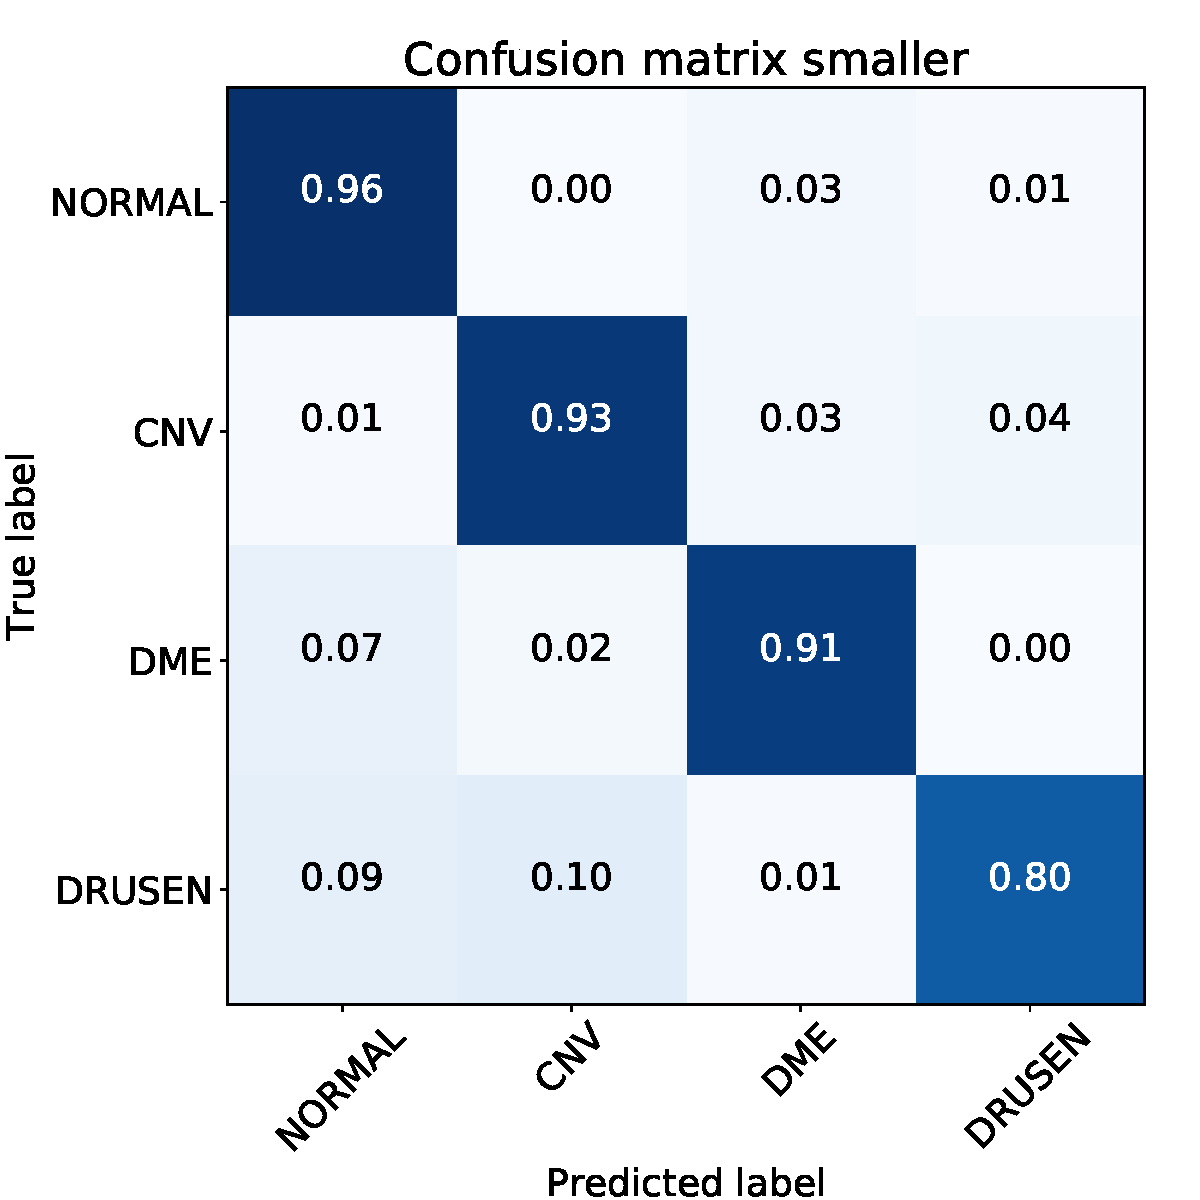
\includegraphics[width=0.4\linewidth]{Plots/confusion_matrix_smaller.pdf}}
  \subcaptionbox{Verteilung des Outputs des Netzes für ein Validierungssample\label{fig:out}}{\centering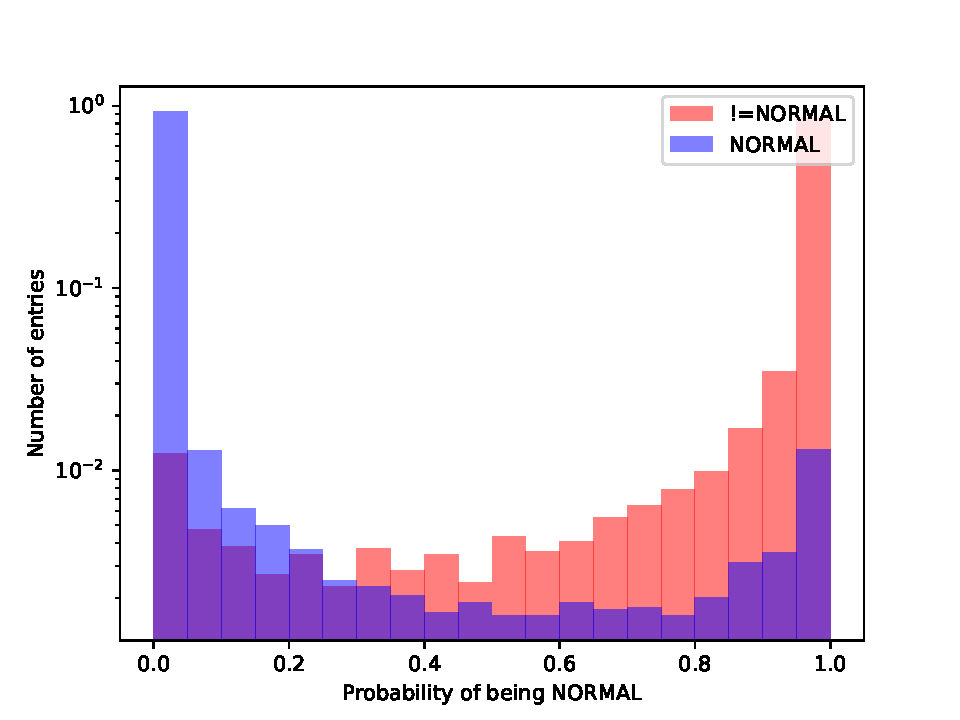
\includegraphics[width=0.55\linewidth]{Plots/NORMAL_or_not_log_smaller.pdf}}
  \caption{Die Verwirrungsmatrix \protect\subref{fig:conf}, sowie der Output \protect\subref{fig:out} der Hauptarchitektur des CNN. Die Verwirrungsmatrix zeigt sehr hohe Genauigkeiten für die einzelnen Klassen. Der Output des Netzes zeigt ebenfalls eine gute Trennung der Krankheiten vom gesunden Auge.}
  \label{fig:erg}
\end{figure}
%
Allerdings zeigt diese Arbeit auch, dass sich mit deutlich einfacheren
Architekturen funktionierende Modelle entwickeln lassen. Insbesondere zeigt
sich trotz starker Skalierung des Datensatzes, was eine deutliche Steigerung
der \textit{computing performance} zur Folge hat, eine Lösung mit einem
einfachen vollständig vernetzten Netz. Dabei ist eine Genauigkeit von etwa
$\SI{73}{\percent}$ möglich. Dies liegt deutlich unterhalb dessen, was das CNN
leisten kann.
%
\begin{figure}[h!]
  \subcaptionbox{Verwirrungsmatrix\label{fig:conf_alt}}{\centering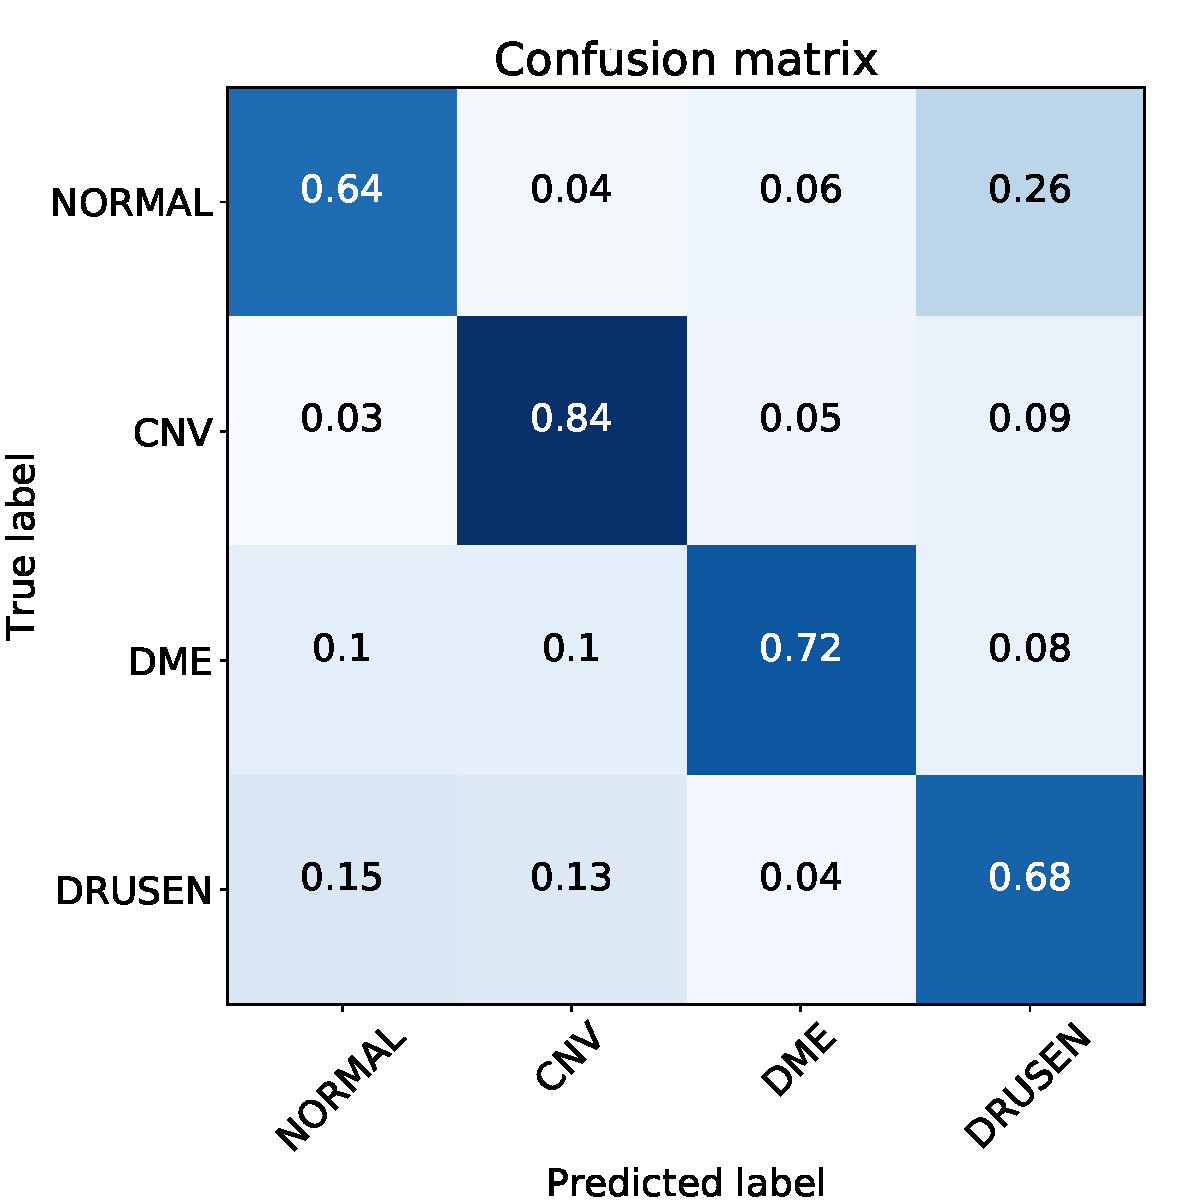
\includegraphics[width=0.4\linewidth]{Plots/confusionmatrix6test.pdf}}
  \subcaptionbox{Verlauf der Genauigkeit\label{fig:acc_alt}}{\centering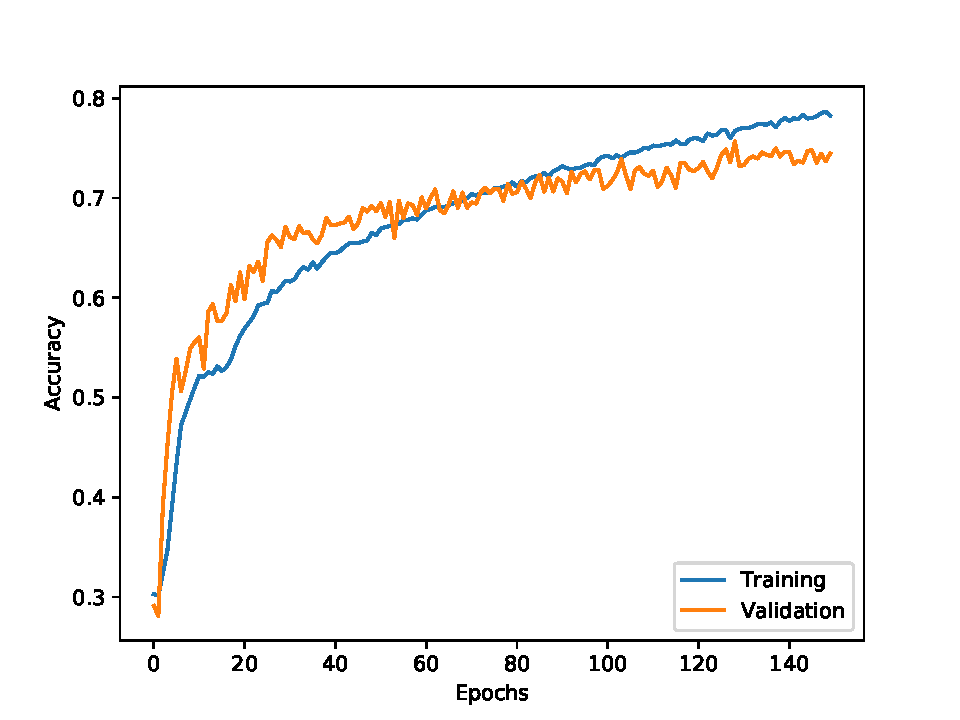
\includegraphics[width=0.55\linewidth]{Plots/accuracyhistory6.pdf}}
  \caption{Die Verwirrungsmatrix \protect\subref{fig:conf_alt}, sowie der Verlauf der Genauigkeit \protect\subref{fig:acc_alt} während des Trainings der Alternativmethode. Die Verwirrungsmatrix zeigt deutlich geringere Genauigkeiten als das CNN. Der Verlauf der Genauigkeit zeigt, dass ein längeres Trainieren ins overtraining führt.}
  \label{fig:erg}
\end{figure}
%
Auch für die Alternativmethode zeigt sich in Abbildung~\ref{fig:conf}, dass die
Unterscheidung der Klasse DRUSEN von den Klassen NORMAL und CNV besonders
schwierig erscheint. Allerdings scheint die Präparation der Daten wie in
Abschnitt~\ref{sec:alter} beschrieben, dafür zu sorgen, dass insbesondere auch
gesunde Retinas in etwa $\SI{25}{\percent}$ der Fälle für DRUSEN gehalten
werden.
